\usepackage{listings}

\section{Experiments}
\

In this section, we designed a simple simulation experiment to verify the effectiveness of our proposed method. We input six data files, categorized into three types: non-plagiarism, explicit plagiarism, and implicit plagiarism. Each category is further divided into original texts and plagiarized texts. The experimental procedure is illustrated in the following diagram:
\begin{figure}[h]
    \centering
    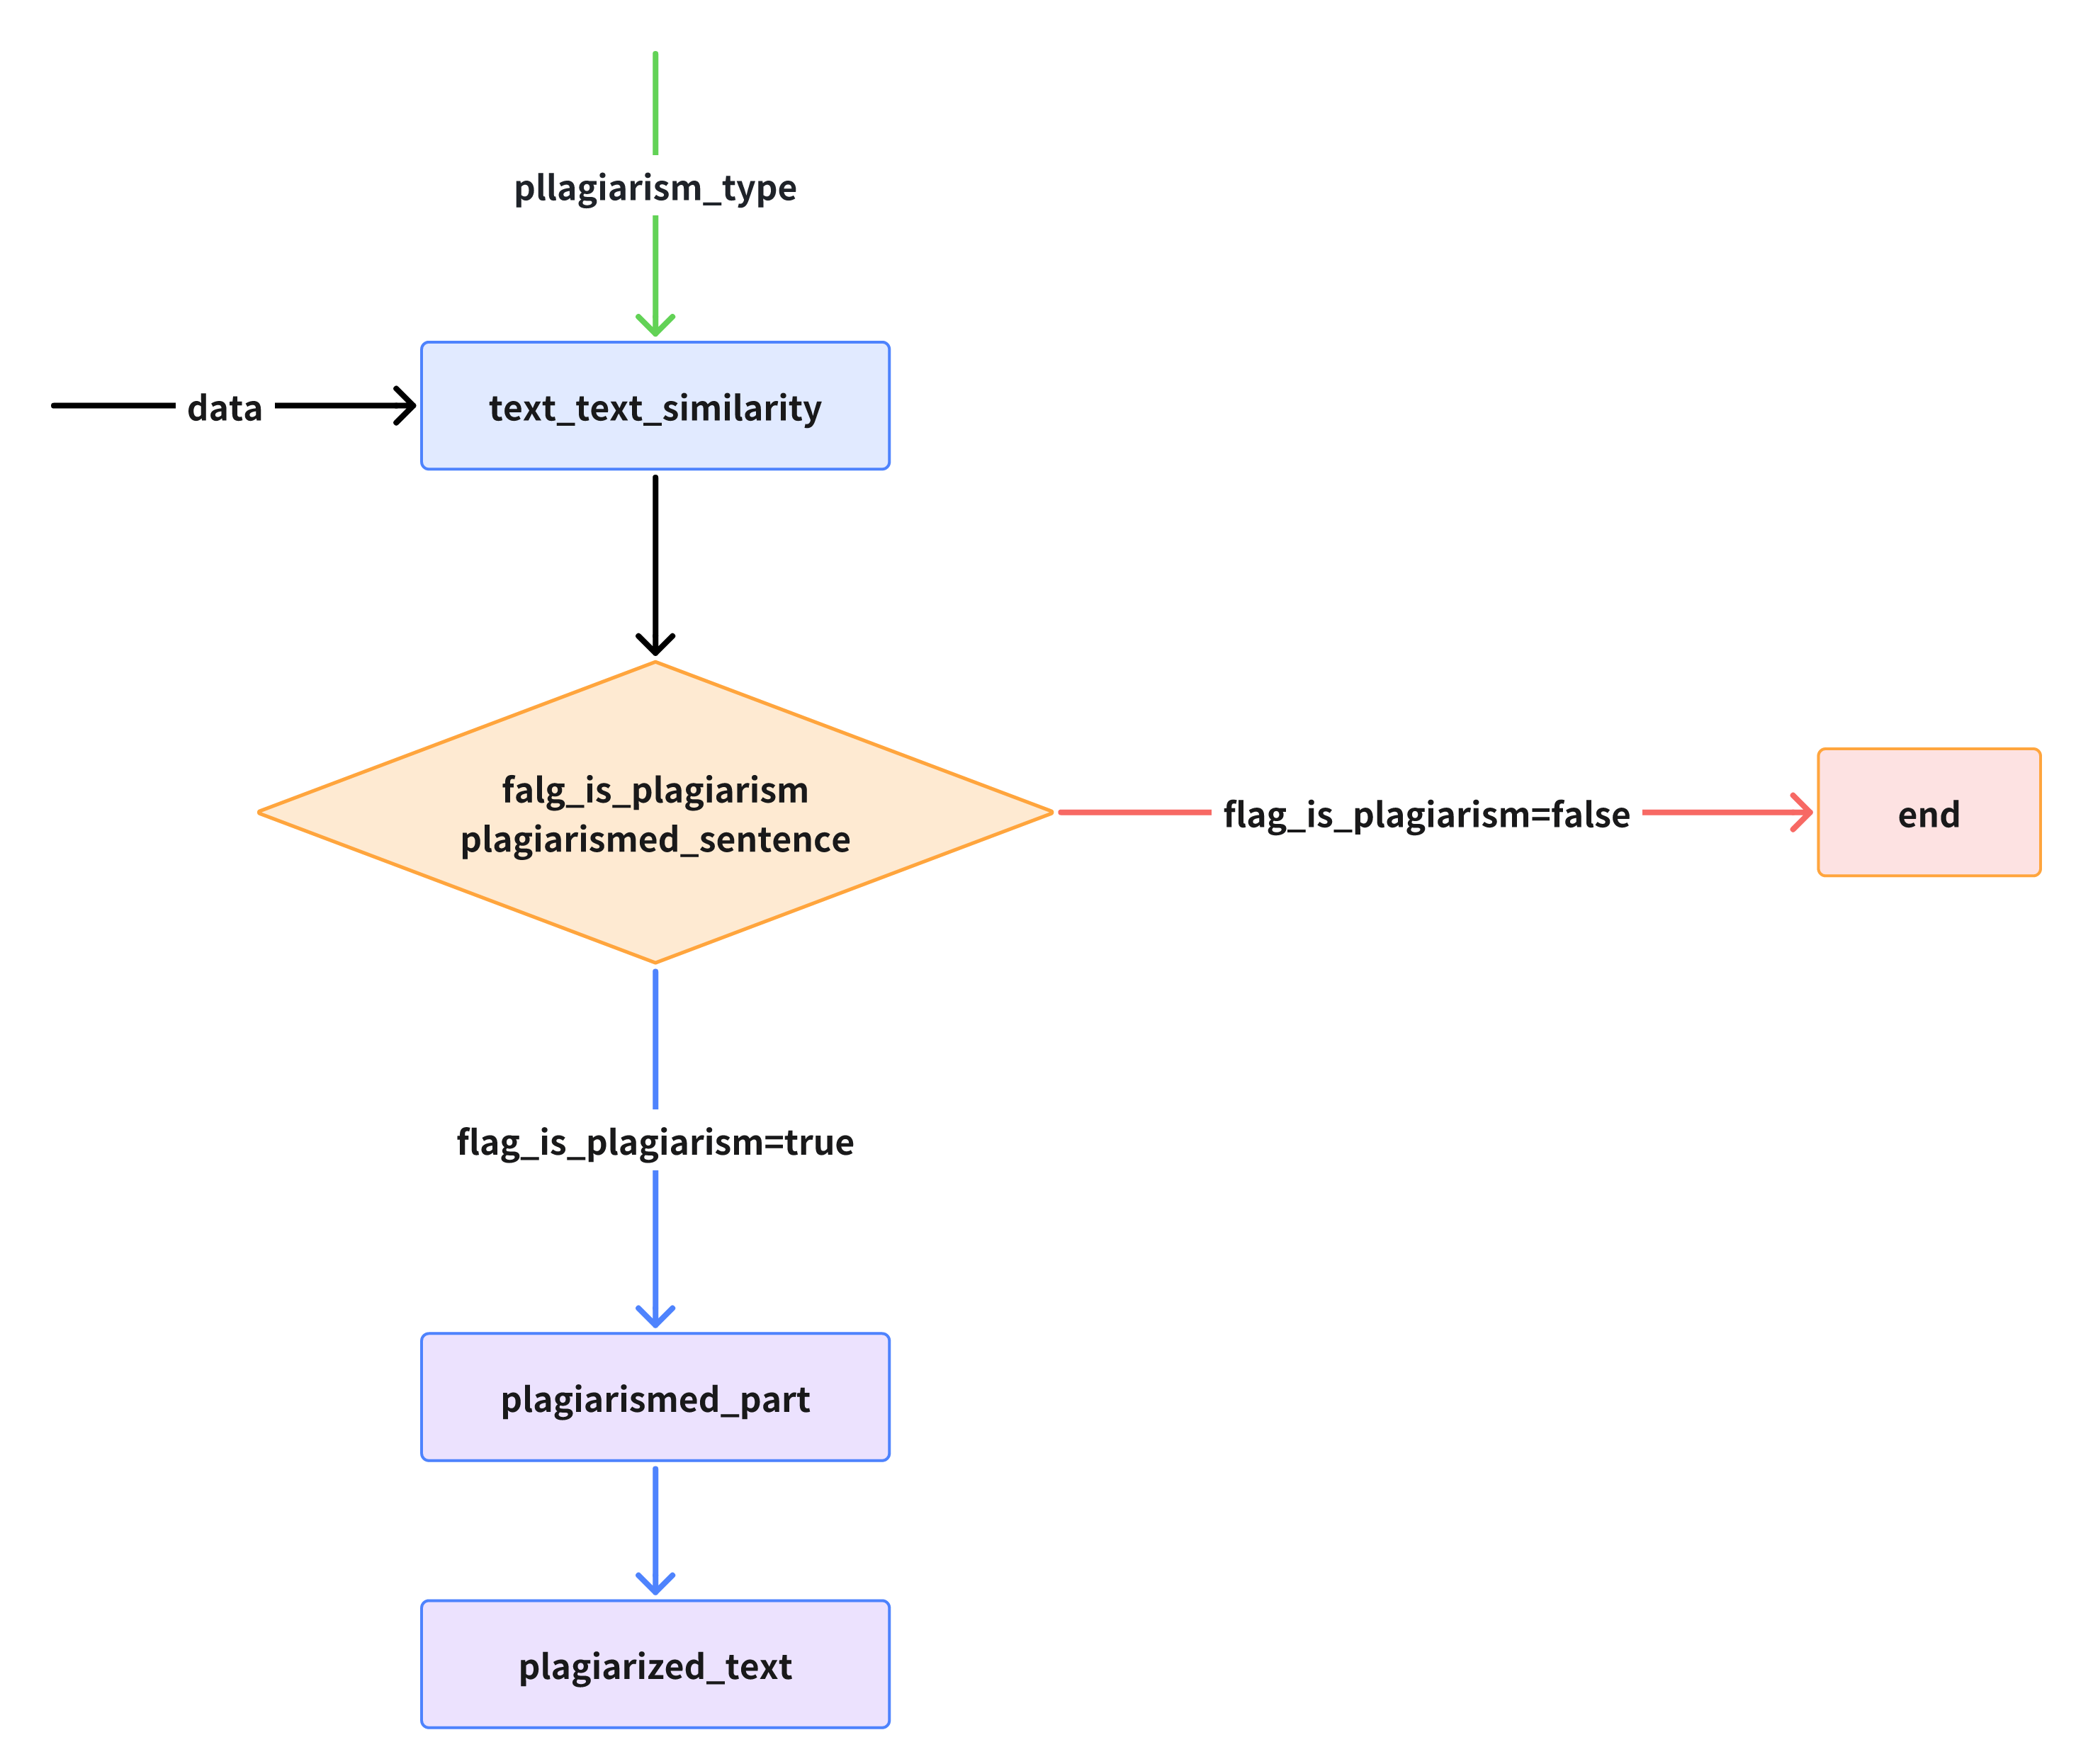
\includegraphics[width=1\linewidth]{png/system.png}
    \caption{system framework}
    \label{fig:2}
\end{figure}

Below are the steps for a simple experiment, where you can see the detailed process of how we conducted it.

\subsection{Input}
\textbf{Input}:QuerySentence = "I enjoy playing basketball with my friends. We play every weekend."

Our goal is to find the text most similar to this sentence in our corpus.

\subsection{Similarity Retrieval}
\

In this section, our goal is to retrieve the three text segments from the corpus that are most semantically similar to the query sentence. The core of this process lies in calculating the similarity between the query sentence and each text in the corpus, ranking them by similarity scores, and selecting the top three most relevant segments. Cosine similarity is used as the measure for similarity. Before computation, the texts are converted into vector embeddings using SentenceTransformer.

So now we get the ouput:
Most similar sentences:\\
1. He enjoy playing basketball with my friends. They play every weekend. (Similarity: 0.5823)\\
2. Friendship makes life more enjoyable. It adds meaning to our lives. (Similarity: 0.3458)\\
3. I am learning to play the guitar. It's a challenging but rewarding hobby. (Similarity: 0.3156)\\
Plagiarism has occurred\\
Query: I enjoy playing basketball with my friends. We play every weekend.\\
Most similar sentences: He enjoy playing basketball with my friends. They play every weekend.

\subsection{Get the most similar text}
\

In the previous section, we identified the most similar texts based on cosine similarity, and if the similarity exceeded 0.5, we considered the possibility of plagiarism. In this section, we attempt to more accurately identify the potential plagiarized parts.

Specifically, we first split all the texts into individual sentences. Next, we divide the text data into two categories: the original text dataset and the plagiarized text dataset. For each sentence in the plagiarized dataset, we compare it with every sentence in the original text dataset, calculate their similarities, and find the most similar sentence. Through this method, we can not only identify the similarity between two sentences but also precisely locate the parts where plagiarism is most likely involved.

\textbf{Ouput}:\\
The most likely plagiarized text is:\\
We play every weekend.\\
They play every weekend.\\
Their similarity is: 0.8143205